\documentclass[12pt,letterpaper]{article}
\usepackage[utf8]{inputenc}
\usepackage[T1]{fontenc}
% NewTX reproduce la referencia; Times es la alternativa de TeX Live mínimo.
\IfFileExists{newtxtext.sty}{\usepackage{newtxtext}\usepackage{newtxmath}}{\usepackage{mathptmx}}
\usepackage[letterpaper,top=2.5cm,bottom=2.5cm,left=3cm,right=3cm,footskip=1.25cm]{geometry}
\usepackage{setspace,ragged2e}
\onehalfspacing
\usepackage{microtype}
\usepackage{xcolor}
\usepackage{array,tabularx,booktabs,longtable}
\usepackage{tikz}
\usetikzlibrary{arrows.meta,positioning,fit,backgrounds,calc}
\usepackage[hidelinks]{hyperref}
% Los nombres se conservan para los diagramas, ahora en escala de grises.
\definecolor{Azul}{gray}{0}
\definecolor{Oro}{gray}{0.35}
\definecolor{Marfil}{gray}{0.97}
\definecolor{Arena}{gray}{0.92}
\definecolor{Gris}{gray}{0.25}
\hypersetup{pdftitle={Plataforma universitaria: fases 1 y 2},pdfsubject={Cómputo en la Nube},pdfauthor={Equipo académico por completar}}
\urlstyle{same}
\renewcommand{\contentsname}{Índice}
\renewcommand{\refname}{Fuentes consultadas}
\renewcommand{\figurename}{Figura}
\renewcommand{\tablename}{Tabla}
\renewcommand{\arraystretch}{1.22}
\setlength{\tabcolsep}{5pt}
\setlength{\parindent}{1.25cm}
\setlength{\parskip}{0pt}
\setlength{\emergencystretch}{4em}
\setcounter{tocdepth}{1}
\newcolumntype{Y}{>{\raggedright\arraybackslash}X}
\newcolumntype{P}[1]{>{\raggedright\arraybackslash}p{#1}}
\AddToHook{env/tabularx/before}{\noindent}
\newcommand{\codigo}[1]{\texttt{\small #1}}
\newcommand{\apartado}[1]{\section{#1}}
\newcommand{\destacado}[2]{\subsection*{#1}#2\par}
\raggedbottom
\makeatletter
% Mismo formato de títulos y pie que la referencia, sin paquetes adicionales.
\renewcommand{\section}{\@startsection{section}{1}{0pt}{-18pt}{12pt}{\normalfont\bfseries\large}}
\renewcommand{\subsection}{\@startsection{subsection}{2}{0pt}{-15pt}{9pt}{\normalfont\bfseries\normalsize}}
\renewcommand{\@seccntformat}[1]{\csname the#1\endcsname.\hspace{0.6em}}
\def\ps@academico{%
  \def\@oddhead{}\def\@evenhead{}%
  \def\@oddfoot{\vbox{\hrule height 0.4pt\kern6pt\hbox to\textwidth{\normalfont\small\PieInstitucional\hfil\thepage}}}%
  \let\@evenfoot\@oddfoot}
\makeatother
% Editar estos campos. No se incluyen nombres ni afiliaciones supuestos.
\newcommand{\Institucion}{[Nombre de la institución]}
\newcommand{\Plantel}{[Facultad, escuela o plantel]}
\newcommand{\Asignatura}{Cómputo en la Nube}
\newcommand{\Integrantes}{[Nombre(s) de integrante(s)]}
\newcommand{\Profesor}{[Nombre del profesor o profesora]}
\newcommand{\Grupo}{[Grupo]}
\newcommand{\FechaEntrega}{2 de noviembre de 2026}
\newcommand{\TituloProyecto}{Plataforma universitaria de estudio}
\newcommand{\VersionInforme}{1.0 documental}

\hypersetup{pdfauthor={\AutoresPDF}}
\pagestyle{academico}
\begin{document}
\begin{titlepage}
\thispagestyle{empty}
\begin{tikzpicture}[remember picture,overlay]
\fill[Azul] (current page.north west) rectangle ([yshift=-4.2cm]current page.north east);
\fill[Oro] ([yshift=-4.2cm]current page.north west) rectangle ([yshift=-4.45cm]current page.north east);
\fill[Arena] ([xshift=-1.2cm,yshift=1.2cm]current page.south east) rectangle ([xshift=-4cm,yshift=4cm]current page.south east);
\draw[Azul,line width=1.4pt] ([xshift=-1.5cm,yshift=1.5cm]current page.south east) rectangle ([xshift=-4.3cm,yshift=4.3cm]current page.south east);
\node[anchor=north west,align=left,text width=16cm,text=white,font=\Large\bfseries] at ([xshift=2.15cm,yshift=-1.1cm]current page.north west) {\Institucion};
\node[anchor=north west,align=left,text width=16cm,text=white,font=\large] at ([xshift=2.15cm,yshift=-2.25cm]current page.north west) {\Plantel};
\end{tikzpicture}\par
\vspace*{2.7cm}
{\color{Azul}\small\bfseries INFORME ACADÉMICO\par}
\vspace{0.5cm}
{\color{Azul}\Huge\bfseries\TituloProyecto\par}
\vspace{0.4cm}
{\LARGE Arquitectura cloud y desarrollo inicial\par}
\vspace{0.3cm}
{\Large Fase 1: base técnica y viabilidad\par Fase 2: espacio académico\par}
\vspace{0.8cm}
\textcolor{Oro}{\rule{0.36\linewidth}{3pt}}\par
\vspace{0.6cm}
\begin{tabularx}{\linewidth}{P{2.6cm}Y}
\textbf{Asignatura} & \Asignatura\\
\textbf{Integrantes} & \Integrantes\\
\textbf{Profesor(a)} & \Profesor\\
\textbf{Grupo} & \Grupo\\
\textbf{Fecha} & \FechaEntrega\\
\end{tabularx}
\vfill
\begin{minipage}{0.68\linewidth}
\small\textcolor{Gris}{Versión \VersionInforme. El informe distingue diseño, implementación y verificación. Los campos académicos son editables; la portada no afirma afiliación oficial ni utiliza escudos institucionales.}
\end{minipage}
\end{titlepage}
\setcounter{page}{2}

\justifying
\setlength{\parindent}{1.25cm}
\apartado{Motivación y propuesta de valor}
\textbf{Resumen.} Se propone una plataforma web para estudiantes universitarios de ciencias físico-matemáticas e ingeniería que reúna organización académica, tutoría con IA y práctica. Este informe documenta las dos primeras etapas: H0, base técnica y pruebas de viabilidad; y H1, espacio académico. Google Cloud es la plataforma propuesta para persistencia, identidad, procesamiento asíncrono y ejecución administrada. El proveedor de IA previsto es DeepSeek. La integración completa del tutor corresponde a etapas posteriores.

\subsection*{Problema y motivación}
Un estudiante puede tener apuntes en archivos, fechas en otra aplicación y dudas en un chat que no conoce el contexto de su materia. Además, recibir una explicación no siempre permite comprobar si comprendió un concepto. El proyecto busca conectar estas actividades para facilitar el estudio y ofrecer oportunidades de explorar, practicar y reconocer dificultades. Esta necesidad se plantea como hipótesis de diseño que deberá contrastarse con estudiantes.

\destacado{Presentación del proyecto}{Queremos que un estudiante pueda entrar a su espacio académico, ubicar sus pendientes y estudiar a partir de sus propios apuntes. Desde ahí podrá pedir una explicación con fuentes, explorar un concepto mediante un recurso interactivo y practicar para reconocer qué necesita reforzar. La nube permitirá conservar su trabajo entre sesiones y procesar materiales sin interrumpir la navegación. La propuesta conecta \textbf{organización, comprensión y práctica} en un mismo recorrido, con preferencias ajustables y progreso explicable.}

\subsection*{Diferenciación buscada}
Se priorizarán el material, método y notación del alumno; el tutor podrá crear experiencias interactivas variadas y distinguir entre ayuda solicitada y evidencia independiente. Su personalidad se elegirá por separado del tipo de apoyo: el estudiante podrá pedir pistas o una solución completa. El pasaporte y la comparación entre amigos serán voluntarios. Estos atributos orientan el diseño; no constituyen una afirmación de superioridad frente a herramientas no evaluadas.

\subsection*{Objetivo y alcance}
Diseñar e iniciar una plataforma cloud con identidad, organización académica y contratos de integración reproducibles. H0/H1 cubren la base y el espacio de materias, temas, periodos, pendientes y horarios. Las materias son libres; cálculo, física, álgebra lineal y programación servirán como casos de validación. No se promete mejora de calificaciones ni se sustituye al profesor.

\apartado{Fundamento cloud y decisiones de arquitectura}
La aplicación se plantea como un servicio web para el estudiante. El equipo combinará servicios administrados para reducir la operación de servidores y concentrarse en las funciones educativas. La clasificación de servicio se apoya en la definición de cloud del NIST [1].

\begin{tabularx}{\linewidth}{P{3cm}Y Y}
\toprule
\textbf{Servicio propuesto} & \textbf{Responsabilidad} & \textbf{Concepto cloud aplicado}\\
\midrule
Cloud Run & Web, API y worker en contenedores. & Ejecución administrada y ajuste de capacidad.\\
Firebase Auth & Identidad del estudiante. & Autenticación administrada.\\
Firestore & Perfiles, materias, agenda y estados. & Persistencia documental independiente de instancias.\\
Cloud Storage & Originales, páginas e índices privados. & Almacenamiento de objetos.\\
Cloud Tasks & Entrega de trabajos al worker. & Desacoplamiento y reintentos.\\
Secret Manager & Credenciales del proveedor de IA. & Separación de secretos y código.\\
Logging y Monitoring & Errores, latencias y trabajo pendiente. & Observabilidad y operación.\\
\bottomrule
\end{tabularx}

\subsection*{Identidad, datos y permisos}
Firebase Auth identifica a la persona; la API valida su token y comprueba que puede acceder al recurso. IAM controla lo que los servicios pueden hacer en GCP. Son dos fronteras distintas: estar autenticado no concede acceso a todas las materias y una identidad de servicio no reemplaza la autorización del estudiante.

Firestore contendrá registros consultables; Storage conservará archivos grandes. Los documentos se mantendrán privados y las cargas utilizarán autorizaciones temporales, verificando tipo y tamaño antes de procesar. Las claves del proveedor permanecerán en backend. El renderer tendrá un origen separado y capacidades limitadas.

\subsection*{Operación y costo}
Se parte del Free Tier, sin créditos trial. Las cuotas, servicios habilitados, región y facturación deberán comprobarse antes de desplegar [8]. Se limitarán instancias, concurrencia y trabajos, y se medirán almacenamiento, tráfico y consumo de IA. Las alertas presupuestarias por sí solas no detienen el gasto [9]. Se requieren resultados reales para afirmar escalamiento, disponibilidad o costo observado.

\apartado{Arquitectura propuesta y flujo de información}
La figura representa el destino arquitectónico de la v1. Las fases H0 y H1 desarrollan la base y el espacio académico; los componentes de IA, cola y almacenamiento documental se muestran para explicar sus relaciones futuras, sin atribuirles implementación completa.

\begin{center}
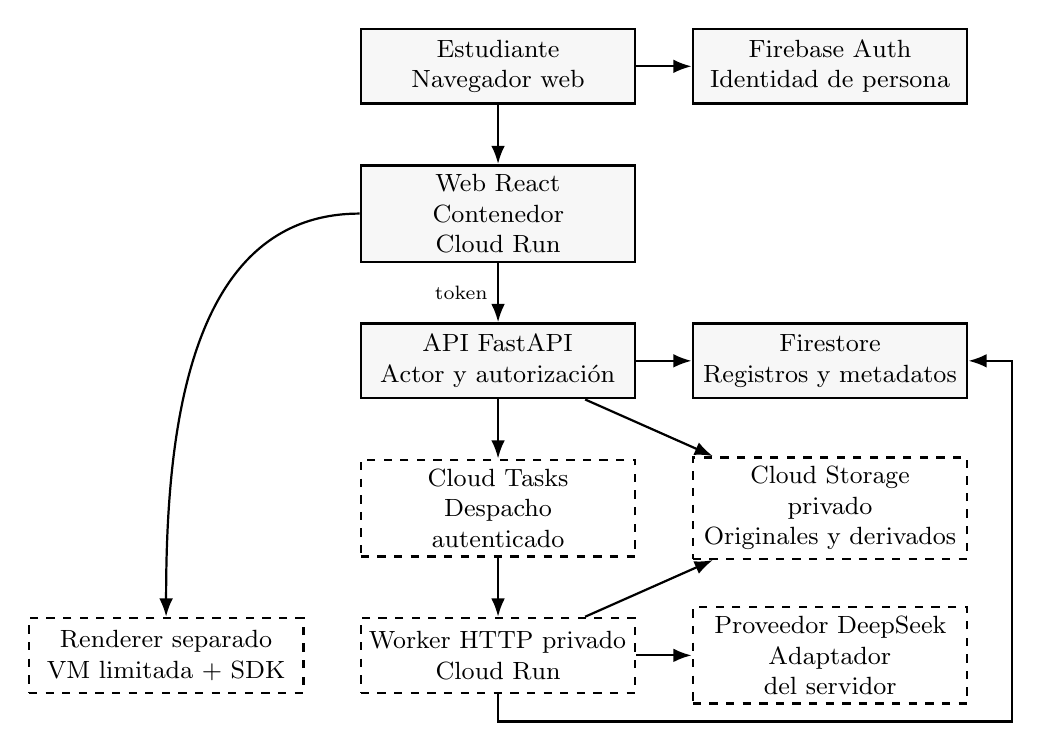
\begin{tikzpicture}[>=Latex,node distance=0.75cm and 0.7cm,
 box/.style={draw=Azul,line width=0.9pt,fill=Marfil,align=center,minimum height=0.95cm,text width=3.25cm,font=\small},
 future/.style={box,dashed,fill=white},arr/.style={->,draw=Azul,thick}]
\node[box] (user) {Estudiante\\Navegador web};
\node[box,right=of user] (auth) {Firebase Auth\\Identidad de persona};
\node[box,below=of user] (web) {Web React\\Contenedor Cloud Run};
\node[box,below=of web] (api) {API FastAPI\\Actor y autorización};
\node[box,right=of api] (db) {Firestore\\Registros y metadatos};
\node[future,below=of api] (tasks) {Cloud Tasks\\Despacho\\autenticado};
\node[future,right=of tasks] (store) {\mbox{Cloud Storage}\\privado\\Originales y derivados};
\node[future,below=of tasks] (worker) {Worker HTTP privado\\Cloud Run};
\node[future,right=of worker] (ai) {Proveedor DeepSeek\\Adaptador del servidor};
\node[future,left=of worker] (renderer) {Renderer separado\\VM limitada + SDK};
\draw[arr] (user)--(web);
\draw[arr] (user)--(auth);
\draw[arr] (web)--node[left,font=\scriptsize]{token}(api);
\draw[arr] (api)--(db);
\draw[arr] (api)--(tasks);
\draw[arr] (tasks)--(worker);
\draw[arr] (api)--(store);
\draw[arr] (worker)--(store);
\draw[arr] (worker)--(ai);
\draw[arr] (worker.south) -- ++(0,-0.35) -| ([xshift=0.55cm]db.east) -- (db.east);
\draw[arr] (web.west) to[out=180,in=90] (renderer.north);
\end{tikzpicture}
\end{center}
\begin{center}\small\textbf{Figura 1.} Arquitectura de destino. Trazo discontinuo: capacidades de integración posterior. Elaboración propia a partir del plan del proyecto.\end{center}

\subsection{Recorrido síncrono y recorrido diferido}
En H1, el navegador obtiene una sesión y solicita datos al API. El servidor valida el token, habilitación del piloto y pertenencia del recurso. Consulta o modifica registros y devuelve un resultado con revisión y errores definidos. Los datos persistentes no deben depender de la memoria de una instancia de contenedor.

Posteriormente, una operación lenta creará un trabajo persistente. La cola notificará al worker, que verificará el alcance y actualizará el estado. El navegador consultará el progreso: cerrar una pestaña no debe perder el trabajo. Un recurso interactivo autorizado se enviará al renderer en otro origen; ese componente no recibirá secretos ni acceso general a documentos.

\textbf{Fronteras principales:} navegador--API (actor humano), API--datos (propiedad), Tasks--worker (identidad de servicio), servidor--IA (contenido mínimo autorizado) y aplicación--renderer (mensajes acotados). Cada frontera requiere pruebas específicas; una flecha en un diagrama no acredita el permiso.


\apartado{Fase 1 (H0): base técnica y viabilidad}
H0 busca reducir riesgos antes de construir funcionalidades sobre supuestos no comprobados. El stack propuesto combina React/TypeScript para la web y Python/FastAPI para la API y el procesamiento de materiales. Se utilizarán dependencias fijadas, configuración por ambiente y pruebas locales reproducibles.

\begin{tabularx}{\linewidth}{P{1.2cm}Y Y}
\toprule
\textbf{Tarea} & \textbf{Entrega} & \textbf{Criterio de comprobación}\\
\midrule
T01 & Workspace, API mínima, web y renderer. & Instalar desde lockfiles y arrancar los tres servicios.\\
T02 & Esquemas, errores, puertos y cliente generado. & Rechazar entradas indebidas y detectar contratos desactualizados.\\
T03 & Prototipo de laboratorio limitado. & Mostrar tres experiencias y bloquear acceso a capacidades no autorizadas.\\
T04 & Prototipo de extracción y recuperación. & Recuperar fuentes correctas y señalar transcripciones ambiguas.\\
\bottomrule
\end{tabularx}

\subsection*{Contratos y separación de infraestructura}
La API define tipos compartidos de materia, fuente, trabajo y error. El cliente TypeScript se genera desde esos esquemas para evitar mantener dos versiones manuales. Los campos controlados por servidor, como propietario y resultados, no se aceptan en entradas de creación. Las fechas y la zona horaria deben ser explícitas.

Los puertos permiten sustituir almacenamiento, cola y proveedor sin cambiar las reglas del dominio. Los dobles locales sirven para pruebas; no demuestran que Firestore, Cloud Tasks o DeepSeek estén integrados. El código pendiente debe responder como pendiente, sin simular éxito.

\subsection*{Pruebas de viabilidad}
El laboratorio interpretará JavaScript en un runtime limitado y expondrá únicamente operaciones visuales autorizadas. Se probarán un explorador matemático, una simulación física y una visualización de algoritmo. Los controles deberán impedir acceso a credenciales y datos privados, además de limitar ejecución y memoria.

La extracción cubrirá PDF, PPTX, notas e imágenes. Cada bloque conservará localizador de página o diapositiva. La recuperación buscará dentro de la materia y fuentes elegidas; las fórmulas dudosas se enviarán a revisión. La visión y calidad del proveedor requieren pruebas reales con credencial y corpus conocido. El cierre de H0 depende también de estas validaciones, no solo del arranque local.

\apartado{Fase 2 (H1): espacio académico}
H1 construirá el recorrido que el estudiante utiliza antes de conversar con la IA. La entrada principal mostrará materias y pendientes; el chat permanecerá cerrado hasta que el usuario lo abra. Se busca una primera sesión breve, con datos opcionales y posibilidad de completar la organización después.

\begin{tabularx}{\linewidth}{P{1.2cm}Y Y}
\toprule
\textbf{Tarea} & \textbf{Entrega} & \textbf{Criterio de comprobación}\\
\midrule
T05 & Sistema visual y navegación adaptable. & Uso móvil/teclado y legibilidad.\\
T06 & Identidad y autorización del piloto. & Rechazar sesión inválida y acceso a datos ajenos.\\
T07 & Periodos, materias y temas. & Crear una materia libre y editarla conservando relaciones.\\
T08 & Inicio, pendientes y horarios. & Fechas coherentes y datos persistentes al recargar.\\
\bottomrule
\end{tabularx}

\subsection*{Organización libre y diseño}
La estructura será perfil, periodo opcional, materia y temas. El alumno podrá crear asignaturas con nombres propios y elegir una ilustración genérica de un catálogo. El dibujo no determina el contenido de la materia. Se incorporarán estados vacíos, carga y error con acciones claras.

La identidad visual se inspira en Block \& Bold, con azul, oro, fondos claros y bloques de borde firme. Se comprobarán contraste, foco visible, objetivos táctiles y reducción de movimiento. El color universitario es inspiración; no se utilizan escudos ni se afirma afiliación institucional.

\subsection*{Acceso y persistencia}
Se utilizarán cuentas internas para probar el piloto. El backend verificará el token y el propietario de cada recurso. Las pruebas con cuentas A, B y C intentarán acceder a materias, agenda y datos ajenos cambiando sus IDs. Las reglas cliente de base y archivos comenzarán restrictivas.

El almacenamiento local de una instancia no será la fuente de verdad del despliegue cloud. La API conservará las reglas y Firestore la información persistente. Las pruebas con emuladores se identificarán como locales; IAM y los servicios reales se verificarán cuando exista un proyecto configurado.

\subsection*{Agenda e inicio}
Los pendientes podrán asociarse a una materia y tener fecha, hora o día completo. Los horarios guardarán hora local y zona, con excepciones sencillas. El inicio utilizará información real y mostrará recomendaciones vacías mientras el módulo de aprendizaje no produzca evidencia.

\apartado{Validación, avance y siguientes pasos}
La construcción se verificará por comportamiento observable, con pruebas de reglas, integración y navegador según el riesgo. Una captura de pantalla no demuestra persistencia; un test con proveedor falso no demuestra calidad de IA ni integración cloud.

\begin{tabularx}{\linewidth}{P{3cm}Y}
\toprule
\textbf{Nivel} & \textbf{Qué debe demostrar}\\
\midrule
Contratos y reglas & Campos permitidos, fechas, aislamiento, idempotencia y errores.\\
Recorrido local & Crear materia, editar ilustración, registrar pendiente y recargar.\\
Servicios reales & Token validado, permisos IAM, persistencia y procesamiento en GCP.\\
Calidad educativa & Fuentes correctas, cálculos comprobables y ambigüedad reconocida.\\
Experiencia & Localizar pendientes, recuperar contexto y usar controles sin ayuda.\\
\bottomrule
\end{tabularx}

\subsection*{Estado de este corte}
H0 y H1 cuentan con implementación y pruebas: contratos generados, extracción de PDF/PPTX e imágenes, recuperación de fuentes, laboratorio limitado, identidad, perfil, materias, temas, periodos, agenda y horario. El navegador verifica guardado y recarga, cambio de ilustración y los recorridos principales. El laboratorio ejecuta tres familias de ejemplos y un recurso nuevo generado por DeepSeek; los intentos de acceso a red y DOM quedan bloqueados.

Se probaron visión y respuestas con DeepSeek usando material sintético. La recuperación acertó los 40 casos del corpus pequeño preparado; este resultado no representa precisión general. En Firebase/Firestore reales se comprobaron creación y lectura de un documento, rechazo de token inválido y rechazo de correo externo o sin verificar. Los fixtures remotos se eliminaron al terminar. Se exige el dominio exacto \texttt{pcpuma.acatlan.unam.mx} y habilitación de piloto. La base autorizada está en \texttt{educloud-1d5de}, región \texttt{us-central1}, con acceso cliente denegado. Cloud Run aún corresponde al despliegue posterior; la aplicación se ejecuta localmente.

\subsection*{Riesgos y conclusión}
Los riesgos principales son errores de transcripción matemática, respuestas sin respaldo, acceso entre cuentas, código generado con capacidades excesivas y consumo cloud no previsto. Se atenderán mediante revisión de fuentes, autorización de backend, runtime acotado y límites operativos.

Estas fases establecen las condiciones para conectar \textbf{apuntes, explicación, experimentación y práctica}. Su valor educativo se evaluará observando tareas y resultados de uso; no se atribuyen mejoras de calificaciones sin evidencia. Los próximos hitos incorporarán tutoría, recursos completos, progreso y pasaporte. El catálogo definitivo de estampillas y el nombre del producto siguen abiertos.

\clearpage
\addcontentsline{toc}{section}{Fuentes consultadas}
\begingroup\small
\begin{thebibliography}{9}
\bibitem{nist} P. Mell y T. Grance. \emph{The NIST Definition of Cloud Computing}, SP 800-145, 2011, sección 2. NIST. \url{https://nvlpubs.nist.gov/nistpubs/Legacy/SP/nistspecialpublication800-145.pdf}.
\bibitem{cloud-run} Google Cloud. \emph{What is Cloud Run}, apartados sobre servicios, escalamiento a cero y facturación. \url{https://docs.cloud.google.com/run/docs/overview/what-is-cloud-run}.
\bibitem{firebase-token} Firebase. \emph{Verify ID Tokens}, verificación mediante Admin SDK. \url{https://firebase.google.com/docs/auth/admin/verify-id-tokens}.
\bibitem{firestore-iam} Google Cloud. \emph{Security for server client libraries}, acceso mediante IAM. \url{https://docs.cloud.google.com/firestore/native/docs/security/iam}.
\bibitem{signed-url} Google Cloud. \emph{Signed URLs}, alcance temporal del acceso. \url{https://docs.cloud.google.com/storage/docs/access-control/signed-urls}.
\bibitem{cloud-tasks} Google Cloud. \emph{Create HTTP target tasks programmatically}, autenticación del destino HTTP. \url{https://docs.cloud.google.com/tasks/docs/creating-http-target-tasks}.
\bibitem{logging} Google Cloud. \emph{Structured logging}, campos y carga JSON. \url{https://docs.cloud.google.com/logging/docs/structured-logging}.
\bibitem{free-tier} Google Cloud. \emph{Free Google Cloud features and trial offer}, apartado Google Cloud Free Tier. Se usa la información de cuotas permanentes; se excluye el crédito trial del proyecto. \url{https://docs.cloud.google.com/free/docs/free-cloud-features}.
\bibitem{budgets} Google Cloud. \emph{Create, edit, or delete budgets and budget alerts}, distinción entre presupuestos Alerts-only y Spend cap. \url{https://docs.cloud.google.com/billing/docs/how-to/budgets}.
\end{thebibliography}
\endgroup
\textbf{Fecha de consulta de las fuentes web:} 2 de noviembre de 2026. La disponibilidad, precios, cuotas y cobertura deben comprobarse de nuevo antes de aprovisionar. No se incorporan tarifas numéricas no medidas al informe.

\textbf{Base documental interna:} plan v1, especificación del 2 de noviembre de 2026, arquitectura y contratos, y tareas T01--T08 con hitos H0/H1 del plan de implementación. Estos documentos proporcionan requisitos y propuestas; no son fuentes de evidencia de ejecución. El registro de avance del repositorio conserva los resultados de pruebas.

\end{document}
